
\begin{lemma}
Any periodic signal x(t) with period $T_0$ can be written as 
\begin{equation}
    x(t) = \sum_{n=-\infty}^{\infty} a_n \exp \brak{\frac{\j2\pi nt}{T_0}}\label{ec/1999/2/1/analysis}
\end{equation}
where, $a_n$ is given by
\begin{equation}
    a_n = \frac{1}{T_0}\int_{T_0}x(t)\exp\brak{-\frac{\j2\pi nt}{T_0}}dt\label{ec/1999/2/1/synthesis}
\end{equation}
\end{lemma}
From the given information,
\begin{align}
s(t) = \delta(t), -\frac{T_0}{2} < t < \frac{T_0}{2}
\end{align}
Hence, 
\begin{align}
a_n &= \frac{1}{T_0}\int_{-\frac{T_0}{2}}^{\frac{T_0}{2}}\delta(t)\exp\brak{-\frac{\j2\pi nt}{T_0}}dt\\
        &= \frac{1}{T_0}\\
    \implies s(t) &= \frac{1}{T_0}\sum_{n=-\infty}^{\infty}\exp\brak{\frac{\j2\pi nt}{T_0}}\label{ec/1999/2/1/series}
\end{align}
Therefore option (d) is the correct option.
\begin{lemma}
The Fourier transform of $\exp \brak{\j2\pi f_0t}$ is $\delta(f-f_0)$.
\end{lemma}
Let $S(f)$ be the Fourier transform of s(t). Then using the above lemma and  \eqref{ec/1999/2/1/series}
\begin{equation}
    S(f) = \frac{1}{T_0}\sum_{n=-\infty}^{\infty}\delta\brak{f-\frac{n}{T_0}}\label{ec/1999/2/1/T_0}
\end{equation}
We can also write equation \eqref{ec/1999/2/1/T_0} by substituting $f_0 = \frac{1}{T_0}$ as
\begin{equation}
    S(f) = \sum_{n=-\infty}^{\infty}f_0\delta\brak{f-nf_0}
\end{equation}
Thus we can observe that the Fourier transform of an impulse train is an impulse train in the frequency domain.
%\begin{figure}
%    \centering
%    \resizebox{\columnwidth}{!}{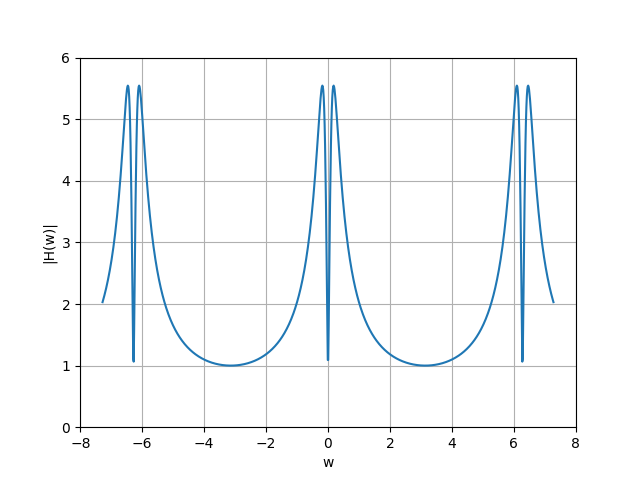
\includegraphics{figures/DTFT.png}}
%    \caption{DTFT of the filter}
%    \label{ec/1999/2/1/DTFT}
%\end{figure}
